\hypertarget{sec-introduction}{%
\chapter{Introduction and Overview}\label{sec-introduction}}

\vspace{-15mm}\addtocontents{toc}{\textit{Lars Kotthoff, Raphael Sonabend, Natalie Foss and Bernd Bischl}}

\textbf{Lars Kotthoff} \newline  \emph{University of Wyoming}

\textbf{Raphael Sonabend} \newline  \emph{Imperial College London}

\textbf{Natalie Foss} \newline  \emph{University of Wyoming}

\textbf{Bernd Bischl} \newline  \emph{Ludwig-Maximilians-Universität
München, and Munich Center for Machine Learning (MCML)}
\newline \newline 

Welcome to the \textbf{M}achine \textbf{L}earning in \textbf{R}
universe. In this book, we will guide you through the functionality
offered by \texttt{mlr3} step by step. If you want to contribute to our
universe, ask any questions, read documentation, or just chat with the
team, head to \url{https://github.com/mlr-org/mlr3} which has several
useful links in the README.

The \href{https://mlr3.mlr-org.com}{\texttt{mlr3}}\index{\texttt{mlr3}}
(Lang et al. 2019) package and the wider \texttt{mlr3} ecosystem provide
a generic, object-oriented\index{object-oriented programming}, and
extensible framework for regression\index{regression}
(Section~\ref{sec-tasks}), classification\index{classification}
(Section~\ref{sec-classif}), and other machine learning
tasks\index{tasks} (Chapter~\ref{sec-special}) for the R language (R
Core Team 2019). On the most basic level, the unified interface provides
functionality to train, test, and evaluate many machine learning
algorithms. You can also take this a step further with hyperparameter
optimization, computational pipelines, model interpretation, and much
more. \texttt{mlr3} has similar overall aims to \texttt{caret} and
\texttt{tidymodels} for R, \texttt{scikit-learn} for Python, and
\texttt{MLJ} for Julia. In general,
\href{https://mlr3.mlr-org.com}{\texttt{mlr3}}\index{\texttt{mlr3}} is
designed to provide more flexibility than other ML frameworks while
still offering easy ways to use advanced functionality. While
\texttt{tidymodels} in particular makes it very easy to perform simple
ML tasks,
\href{https://mlr3.mlr-org.com}{\texttt{mlr3}}\index{\texttt{mlr3}} is
more geared towards advanced ML.

Before we can show you the full power of \texttt{mlr3}, we recommend
installing the
\href{https://mlr3verse.mlr-org.com}{\texttt{mlr3verse}}\index{\texttt{mlr3verse}}
package, which will install several, important packages in the
\texttt{mlr3} ecosystem.

\begin{Shaded}
\begin{Highlighting}[]
\FunctionTok{install.packages}\NormalTok{(}\StringTok{"mlr3verse"}\NormalTok{)}
\end{Highlighting}
\end{Shaded}

\hypertarget{installguide}{%
\section{Installation Guidelines}\label{installguide}}

There are many packages in the \texttt{mlr3} ecosystem that you may want
to use as you work through this book. All our packages can be installed
from GitHub and R-universe\footnote{R-universe is an alternative package
  repository to CRAN. The bit of code below tells R to look at both
  R-universe and CRAN when trying to install packages. R will always
  install the latest version of a package.}; the majority (but not all)
packages can also be installed from CRAN. We recommend adding the
mlr-org R-universe to your R options so you can install all packages
with \texttt{install.packages()}, without having to worry which package
repository it comes from. To do this, install
\href{https://cran.r-project.org/package=usethis}{\texttt{usethis}} and
run the following:

\begin{Shaded}
\begin{Highlighting}[]
\NormalTok{usethis}\SpecialCharTok{::}\FunctionTok{edit\_r\_profile}\NormalTok{()}
\end{Highlighting}
\end{Shaded}

In the file that opens add or change the \texttt{repos} argument in
\texttt{options} so it looks something like the code below (you might
need to add the full code block below or just edit the existing
\texttt{options} function).

\begin{Shaded}
\begin{Highlighting}[]
\FunctionTok{options}\NormalTok{(}\AttributeTok{repos =} \FunctionTok{c}\NormalTok{(}
  \AttributeTok{mlrorg =} \StringTok{"https://mlr{-}org.r{-}universe.dev"}\NormalTok{,}
  \AttributeTok{CRAN =} \StringTok{"https://cloud.r{-}project.org/"}
\NormalTok{))}
\end{Highlighting}
\end{Shaded}

Save the file, restart your R session, and you are ready to go!

If you want the latest development version of any of our packages, run

\begin{Shaded}
\begin{Highlighting}[]
\NormalTok{remotes}\SpecialCharTok{::}\FunctionTok{install\_github}\NormalTok{(}\StringTok{"mlr{-}org/\{pkg\}"}\NormalTok{)}
\end{Highlighting}
\end{Shaded}

with \texttt{\{pkg\}} replaced with the name of the package you want to
install. You can see an up-to-date list of all our extension packages at
\url{https://github.com/mlr-org/mlr3/wiki/Extension-Packages}.

\hypertarget{howtouse}{%
\section{How to Use This Book}\label{howtouse}}

You could read this book cover to cover but you may benefit more from dipping in and out of chapters as suits your needs, we have provided a comprehensive index to help you find relevant pages and sections.
We do recommend reading the first part of the book in its entirety as this will provide you with a complete overview of our basic infrastructure and design, which is used throughout our ecosystem.

We have marked sections that are particularly complex with respect to
either technical or methodological detail and could be skipped on a
first read with the following information box:

\begin{tcolorbox}[enhanced jigsaw, colframe=quarto-callout-note-color-frame, rightrule=.15mm, bottomrule=.15mm, toprule=.15mm, opacityback=0, colback=white, left=2mm, arc=.35mm, breakable, leftrule=.75mm]
\begin{minipage}[t]{5.5mm}
\textcolor{quarto-callout-note-color}{\faInfo}
\end{minipage}%
\begin{minipage}[t]{\textwidth - 5.5mm}

\textbf{This section covers advanced ML or technical
details.}\vspace{2mm}

\end{minipage}%
\end{tcolorbox}

Each chapter includes examples, API references, and explanations of
methodologies. At the end of each part of the book we have included
exercises for you to test yourself on what you have learned; you can
find the solutions to these exercises at
\url{https://mlr3book.mlr-org.com/solutions.html}. We have marked more
challenging (and possibly time-consuming) exercises with an asterisk,
'*'.

If you want more detail about any of the tasks used in this book or
links to all the \texttt{mlr3} dictionaries, please see the appendices
in the online version of the book at
\url{https://mlr3book.mlr-org.com/}.

\hypertarget{reproducibility}{%
\subsubsection*{Reproducibility}\label{reproducibility}}

At the start of each chapter we run \texttt{set.seed(123)} and use
\href{https://cran.r-project.org/package=renv}{\texttt{renv}} to manage package versions, you can find our
lockfile at
\url{https://github.com/mlr-org/mlr3book/blob/main/book/renv.lock}.

\hypertarget{styleguide}{%
\section{mlr3book Code Style}\label{styleguide}}

Throughout this book we will use the following code style:

\begin{enumerate}
\def\labelenumi{\arabic{enumi}.}
\item
  We always use \texttt{=} instead of \texttt{\textless{}-} for
  assignment.
\item
  Class names are in \texttt{UpperCamelCase}
\item
  Function and method names are in \texttt{lower\_snake\_case}
\item
  When referencing functions, we will only include the package prefix
  (e.g., \texttt{pkg::function}) for functions outside the \texttt{mlr3}
  universe or when there may be ambiguity about in which package the
  function lives. Note you can use \texttt{environment(function)} to see
  which namespace a function is loaded from.
\item
  We denote packages, fields, methods, and functions as follows:

  \begin{itemize}
  \tightlist
  \item
    \texttt{package} (highlighted in the first instance)
  \item
    \texttt{package::function()} or \texttt{function()} (see point 4)
  \item
    \texttt{\$field} for fields (data encapsulated in an R6 class)
  \item
    \texttt{\$method()} for methods (functions encapsulated in an R6
    class)
  \item
    \texttt{Class} (for R6 classes primarily, these can be distinguished
    from packages by context)
  \end{itemize}
\end{enumerate}

Now let us see this in practice with our first example.

\hypertarget{mlr3-by-example}{%
\section{mlr3 by Example}\label{mlr3-by-example}}

The \texttt{mlr3} universe includes a wide range of tools taking you
from basic ML to complex experiments. To get started, here is an example
of the simplest functionality -- training a model and making
predictions.

\begin{Shaded}
\begin{Highlighting}[]
\FunctionTok{library}\NormalTok{(mlr3)}
\NormalTok{task }\OtherTok{=} \FunctionTok{tsk}\NormalTok{(}\StringTok{"penguins"}\NormalTok{)}
\NormalTok{split }\OtherTok{=} \FunctionTok{partition}\NormalTok{(task)}
\NormalTok{learner }\OtherTok{=} \FunctionTok{lrn}\NormalTok{(}\StringTok{"classif.rpart"}\NormalTok{)}

\NormalTok{learner}\SpecialCharTok{$}\FunctionTok{train}\NormalTok{(task, }\AttributeTok{row\_ids =}\NormalTok{ split}\SpecialCharTok{$}\NormalTok{train)}
\NormalTok{learner}\SpecialCharTok{$}\NormalTok{model}
\end{Highlighting}
\end{Shaded}

\begin{verbatim}
n= 231 

node), split, n, loss, yval, (yprob)
      * denotes terminal node

1) root 231 129 Adelie (0.441558 0.199134 0.359307)  
  2) flipper_length< 206.5 144  44 Adelie (0.694444 0.298611 0.006944)  
    4) bill_length< 43.05 98   3 Adelie (0.969388 0.030612 0.000000) *
    5) bill_length>=43.05 46   6 Chinstrap (0.108696 0.869565 0.021739) *
  3) flipper_length>=206.5 87   5 Gentoo (0.022989 0.034483 0.942529) *
\end{verbatim}

\begin{Shaded}
\begin{Highlighting}[]
\NormalTok{prediction }\OtherTok{=}\NormalTok{ learner}\SpecialCharTok{$}\FunctionTok{predict}\NormalTok{(task, }\AttributeTok{row\_ids =}\NormalTok{ split}\SpecialCharTok{$}\NormalTok{test)}
\NormalTok{prediction}
\end{Highlighting}
\end{Shaded}

\begin{verbatim}
<PredictionClassif> for 113 observations:
    row_ids     truth  response
          1    Adelie    Adelie
          2    Adelie    Adelie
          3    Adelie    Adelie
---                            
        328 Chinstrap Chinstrap
        331 Chinstrap    Adelie
        339 Chinstrap Chinstrap
\end{verbatim}

\begin{Shaded}
\begin{Highlighting}[]
\NormalTok{prediction}\SpecialCharTok{$}\FunctionTok{score}\NormalTok{(}\FunctionTok{msr}\NormalTok{(}\StringTok{"classif.acc"}\NormalTok{))}
\end{Highlighting}
\end{Shaded}

\begin{verbatim}
classif.acc 
     0.9558 
\end{verbatim}

In this example, we trained a decision tree on a subset of the
\href{https://www.rdocumentation.org/packages/palmerpenguins/topics/penguins}{\texttt{penguins}}
dataset, made predictions on the rest of the data and then evaluated
these with the accuracy measure. In Chapter~\ref{sec-basics} we will
break this down in more detail.

The \texttt{mlr3} interface also lets you run more complicated
experiments in just a few lines of code:

\begin{Shaded}
\begin{Highlighting}[]
\FunctionTok{library}\NormalTok{(mlr3verse)}

\NormalTok{tasks }\OtherTok{=} \FunctionTok{tsks}\NormalTok{(}\FunctionTok{c}\NormalTok{(}\StringTok{"breast\_cancer"}\NormalTok{, }\StringTok{"sonar"}\NormalTok{))}

\NormalTok{glrn\_rf\_tuned }\OtherTok{=} \FunctionTok{as\_learner}\NormalTok{(}\FunctionTok{ppl}\NormalTok{(}\StringTok{"robustify"}\NormalTok{) }\SpecialCharTok{\%\textgreater{}\%} \FunctionTok{auto\_tuner}\NormalTok{(}
    \FunctionTok{tnr}\NormalTok{(}\StringTok{"grid\_search"}\NormalTok{, }\AttributeTok{resolution =} \DecValTok{5}\NormalTok{),}
    \FunctionTok{lrn}\NormalTok{(}\StringTok{"classif.ranger"}\NormalTok{, }\AttributeTok{num.trees =} \FunctionTok{to\_tune}\NormalTok{(}\DecValTok{200}\NormalTok{, }\DecValTok{500}\NormalTok{)),}
    \FunctionTok{rsmp}\NormalTok{(}\StringTok{"holdout"}\NormalTok{)}
\NormalTok{))}
\NormalTok{glrn\_rf\_tuned}\SpecialCharTok{$}\NormalTok{id }\OtherTok{=} \StringTok{"RF"}

\NormalTok{glrn\_stack }\OtherTok{=} \FunctionTok{as\_learner}\NormalTok{(}\FunctionTok{ppl}\NormalTok{(}\StringTok{"robustify"}\NormalTok{) }\SpecialCharTok{\%\textgreater{}\%} \FunctionTok{ppl}\NormalTok{(}\StringTok{"stacking"}\NormalTok{,}
    \FunctionTok{lrns}\NormalTok{(}\FunctionTok{c}\NormalTok{(}\StringTok{"classif.rpart"}\NormalTok{, }\StringTok{"classif.kknn"}\NormalTok{)),}
    \FunctionTok{lrn}\NormalTok{(}\StringTok{"classif.log\_reg"}\NormalTok{)}
\NormalTok{))}
\NormalTok{glrn\_stack}\SpecialCharTok{$}\NormalTok{id }\OtherTok{=} \StringTok{"Stack"}

\NormalTok{learners }\OtherTok{=} \FunctionTok{c}\NormalTok{(glrn\_rf\_tuned, glrn\_stack)}
\NormalTok{bmr }\OtherTok{=} \FunctionTok{benchmark}\NormalTok{(}\FunctionTok{benchmark\_grid}\NormalTok{(tasks, learners, }\FunctionTok{rsmp}\NormalTok{(}\StringTok{"cv"}\NormalTok{, }\AttributeTok{folds =} \DecValTok{3}\NormalTok{)))}

\NormalTok{bmr}\SpecialCharTok{$}\FunctionTok{aggregate}\NormalTok{(}\FunctionTok{msr}\NormalTok{(}\StringTok{"classif.acc"}\NormalTok{))}
\end{Highlighting}
\end{Shaded}

\begin{verbatim}
         task_id learner_id classif.acc
1: breast_cancer         RF      0.9737
2: breast_cancer      Stack      0.9386
3:         sonar         RF      0.8406
4:         sonar      Stack      0.7246
\end{verbatim}

In this (much more complex!) example we chose two tasks and two learners
and used automated tuning to optimize the number of trees in the random
forest learner (Chapter~\ref{sec-optimization}), and a machine learning
pipeline that imputes missing data, collapses factor levels, and stacks
models (Chapter~\ref{sec-pipelines} and
Chapter~\ref{sec-pipelines-nonseq}). We also showed basic features like
loading learners (Chapter~\ref{sec-basics}) and choosing resampling
strategies for benchmarking (Chapter~\ref{sec-performance}). Finally, we
compared the performance of the models using the mean accuracy with
three-fold cross-validation.

You will learn how to do all this and more in this book.

\hypertarget{the-mlr3-ecosystem}{%
\section{\texorpdfstring{The \texttt{mlr3}
Ecosystem}{The mlr3 Ecosystem}}\label{the-mlr3-ecosystem}}

Throughout this book, we often refer to \texttt{mlr3}, which may refer
to the single
\href{https://mlr3.mlr-org.com}{\texttt{mlr3}}\index{\texttt{mlr3}} base
package but usually refers to all packages in our ecosystem, this should
be clear from context. The
\href{https://mlr3.mlr-org.com}{\texttt{mlr3}}\index{\texttt{mlr3}}
\emph{package} provides the base functionality that the rest of the
ecosystem depends on for building more advanced machine learning tools.
Figure~\ref{fig-mlr3verse} shows the packages in our ecosystem that
extend
\href{https://mlr3.mlr-org.com}{\texttt{mlr3}}\index{\texttt{mlr3}} with
capabilities for preprocessing, pipelining, visualizations, additional
learners, additional task types, and much more.

\begin{figure}

{\centering 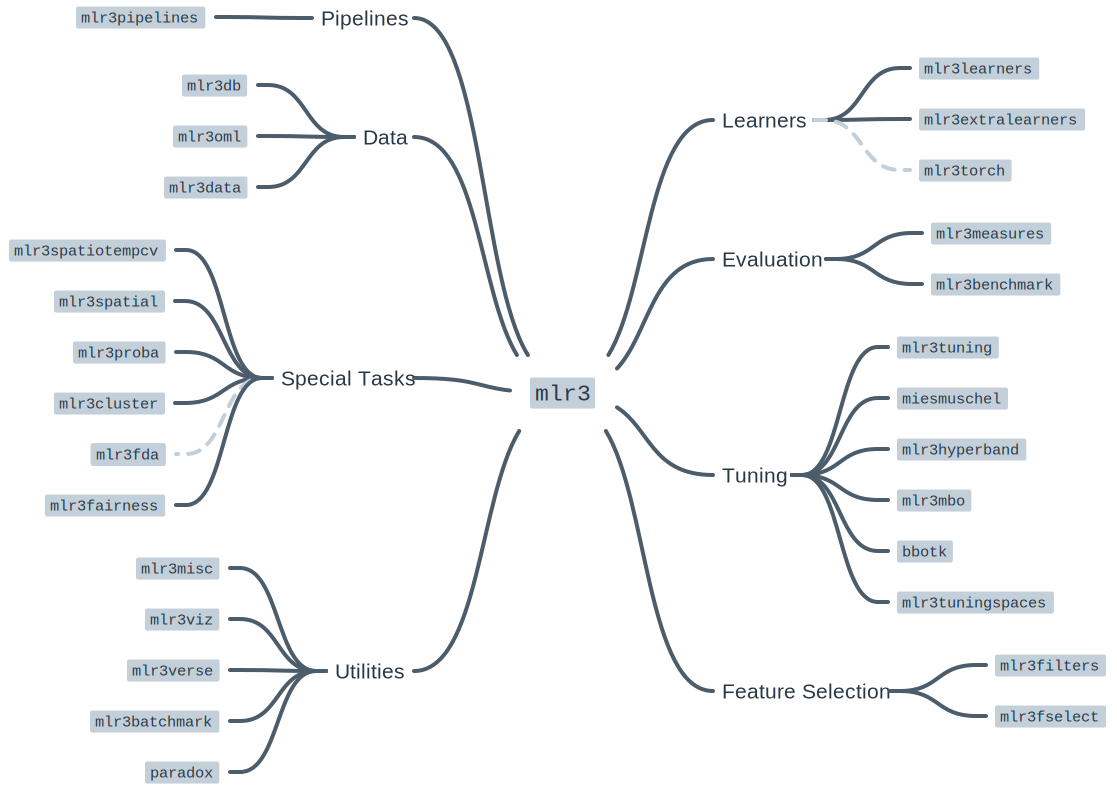
\includegraphics[width=0.8\textwidth,height=\textheight]{chapters/chapter1/Figures/mlr3_ecosystem.png}

}

\caption{\label{fig-mlr3verse}Overview of the \texttt{mlr3} ecosystem,
the packages with gray dashed lines are still in development, all others
have a stable interface.}

\end{figure}

A complete and up-to-date list of extension packages can be found at
\url{https://mlr-org.com/ecosystem.html}.

As well as packages within the \texttt{mlr3} ecosystem, software in the
\texttt{mlr3verse} also depends on the following popular and
well-established packages:

\begin{itemize}
\tightlist
\item
  \href{https://cran.r-project.org/package=R6}{\texttt{R6}}: The class
  system predominantly used in \texttt{mlr3}.
\item
  \href{https://cran.r-project.org/package=data.table}{\texttt{data.table}}:
  High-performance extension of R's \texttt{data.frame}.
\item
  \href{https://cran.r-project.org/package=digest}{\texttt{digest}}:
  Cryptographic hash functions.
\item
  \href{https://cran.r-project.org/package=uuid}{\texttt{uuid}}:
  Generation of universally unique identifiers.
\item
  \href{https://cran.r-project.org/package=lgr}{\texttt{lgr}}:
  Configurable logging library.
\item
  \href{https://cran.r-project.org/package=mlbench}{\texttt{mlbench}}
  and
  \href{https://cran.r-project.org/package=palmerpenguins}{\texttt{palmerpenguins}}:
  Machine learning datasets.
\item
  \href{https://cran.r-project.org/package=future}{\texttt{future}} /
  \href{https://cran.r-project.org/package=future.apply}{\texttt{future.apply}}
  /
  \href{https://cran.r-project.org/package=parallelly}{\texttt{parallelly}}:
  For parallelization (Section~\ref{sec-parallelization}).
\item
  \href{https://cran.r-project.org/package=evaluate}{\texttt{evaluate}}:
  For capturing output, warnings, and exceptions
  (Section~\ref{sec-error-handling}).
\end{itemize}

We build on \href{https://cran.r-project.org/package=R6}{\texttt{R6}}
for object orientation and
\href{https://cran.r-project.org/package=data.table}{\texttt{data.table}}
to store and operate on tabular data. As both are core to \texttt{mlr3}
we \emph{briefly} introduce both packages for beginners; in-depth
expertise with these packages is not necessary to work with
\texttt{mlr3}.

\hypertarget{sec-r6}{%
\subsection{R6 for Beginners}\label{sec-r6}}

\href{https://cran.r-project.org/package=R6}{\texttt{R6}} is one of R's
more recent paradigms for object-oriented
programming\index{object-oriented programming}. If you have experience
with any (class) object-oriented programming then R6 should feel
familiar. We focus on the parts of R6 that you need to know to use
\texttt{mlr3}.

\emph{Objects} are created by constructing an instance of an
\href{https://www.rdocumentation.org/packages/R6/topics/R6Class}{\texttt{R6Class}}
variable using the \texttt{\$new()} initialization method. For example,
say we have implemented a class called \texttt{Foo}, then
\texttt{foo\ =\ Foo\$new(bar\ =\ 1)} would create a new object of class
\texttt{Foo} and set the \texttt{bar} argument of the constructor to the
value \texttt{1}. In practice, we implement a lot of sugar functionality
(Section~\ref{sec-mlr3-utilities}) in \texttt{mlr3} that make
construction and access a bit more convenient.

Some \texttt{R6} objects may have mutable states that are encapsulated
in their \emph{fields}, which can be accessed through the dollar,
\texttt{\$}, operator. Continuing the previous example, we can access
the \texttt{bar} value in the \texttt{foo} object by using
\texttt{foo\$bar} or we could give it a new value,
e.g.~\texttt{foo\$bar\ =\ 2}. These fields can also be `active
bindings', which perform additional computations when referenced or
modified.

In addition to fields, \emph{methods} allow users to inspect the
object's state, retrieve information, or perform an action that changes
the internal state of the object. For example, in \texttt{mlr3}, the
\texttt{\$train()} method of a learner changes the internal state of the
learner by building and storing a model. Methods that modify the
internal state of an object often return the object itself. Other
methods may return a new R6 object. In both cases, it is possible to
`chain' methods by calling one immediately after the other using the
\texttt{\$}-operator; this is similar to the
\texttt{\%\textgreater{}\%}-operator used in \texttt{tidyverse}
packages. For example, \texttt{Foo\$bar()\$hello\_world()} would run the
\texttt{\$bar()} method of the object \texttt{Foo} and then the
\texttt{\$hello\_world()} method of the object returned by
\texttt{\$bar()} (which may be \texttt{Foo} itself).

Fields and methods can be public or private. The public fields and
methods define the API to interact with the object. In \texttt{mlr3},
you can safely ignore private methods unless you are looking to extend
our universe by adding a new class (Chapter~\ref{sec-technical}).

Finally, \texttt{R6} objects are \texttt{environments}, and as such have
reference semantics. This means that, for example, \texttt{foo2\ =\ foo}
does not create a new variable called \texttt{foo2} that is a copy of
\texttt{foo}. Instead, it creates a variable called \texttt{foo2} that
references \texttt{foo}, and so setting \texttt{foo\$bar\ =\ 3} will
also change \texttt{foo2\$bar} to \texttt{3} and vice versa. To copy an
object, use the \texttt{\$clone(deep\ =\ TRUE)} method, so to copy
\texttt{foo}:
\texttt{foo2\ =\ foo\$clone(deep\ =\ TRUE)}{\marginnote{\begin{footnotesize}\texttt{\$clone()}\end{footnotesize}}}.

For a longer introduction, we recommend the \texttt{R6} vignettes found
at \url{https://r6.r-lib.org/}; more detail can be found in
\url{https://adv-r.hadley.nz/r6.html}.

\hypertarget{sec-data.table}{%
\subsection{data.table for Beginners}\label{sec-data.table}}

The package
\href{https://cran.r-project.org/package=data.table}{\texttt{data.table}}
implements
\href{https://www.rdocumentation.org/packages/data.table/topics/data.table-package}{\texttt{data.table()}},
which is a popular alternative to R's \texttt{data.frame()}. We use
\href{https://cran.r-project.org/package=data.table}{\texttt{data.table}}
because it is blazingly fast and scales well to bigger data.

As with \texttt{data.frame}, \texttt{data.table}s can be constructed
with
\href{https://www.rdocumentation.org/packages/data.table/topics/data.table-package}{\texttt{data.table()}}
or
\href{https://www.rdocumentation.org/packages/data.table/topics/as.data.table}{\texttt{as.data.table()}}:

\begin{Shaded}
\begin{Highlighting}[]
\FunctionTok{library}\NormalTok{(data.table)}
\CommentTok{\# converting a matrix with as.data.table}
\FunctionTok{as.data.table}\NormalTok{(}\FunctionTok{matrix}\NormalTok{(}\FunctionTok{runif}\NormalTok{(}\DecValTok{4}\NormalTok{), }\DecValTok{2}\NormalTok{, }\DecValTok{2}\NormalTok{))}
\end{Highlighting}
\end{Shaded}

\begin{verbatim}
       V1     V2
1: 0.8586 0.4891
2: 0.8874 0.7181
\end{verbatim}

\begin{Shaded}
\begin{Highlighting}[]
\CommentTok{\# using data.table}
\NormalTok{dt }\OtherTok{=} \FunctionTok{data.table}\NormalTok{(}\AttributeTok{x =} \DecValTok{1}\SpecialCharTok{:}\DecValTok{6}\NormalTok{, }\AttributeTok{y =} \FunctionTok{rep}\NormalTok{(letters[}\DecValTok{1}\SpecialCharTok{:}\DecValTok{3}\NormalTok{], }\AttributeTok{each =} \DecValTok{2}\NormalTok{))}
\NormalTok{dt}
\end{Highlighting}
\end{Shaded}

\begin{verbatim}
   x y
1: 1 a
2: 2 a
3: 3 b
4: 4 b
5: 5 c
6: 6 c
\end{verbatim}

\texttt{data.table}s can be used much like \texttt{data.frame}s, but
they provide additional functionality that makes complex operations
easier. For example, data can be summarized by groups with a \texttt{by}
argument in the \texttt{{[}} operator and they can be modified in-place
with the \texttt{:=} operator.

\begin{Shaded}
\begin{Highlighting}[]
\CommentTok{\# mean of x column in groups given by y}
\NormalTok{dt[, }\FunctionTok{mean}\NormalTok{(x), by }\OtherTok{=} \StringTok{"y"}\NormalTok{]}
\end{Highlighting}
\end{Shaded}

\begin{verbatim}
   y  V1
1: a 1.5
2: b 3.5
3: c 5.5
\end{verbatim}

\begin{Shaded}
\begin{Highlighting}[]
\CommentTok{\# adding a new column with :=}
\NormalTok{dt[, z }\SpecialCharTok{:}\ErrorTok{=}\NormalTok{ x }\SpecialCharTok{*} \DecValTok{3}\NormalTok{]}
\NormalTok{dt}
\end{Highlighting}
\end{Shaded}

\begin{verbatim}
   x y  z
1: 1 a  3
2: 2 a  6
3: 3 b  9
4: 4 b 12
5: 5 c 15
6: 6 c 18
\end{verbatim}

Finally \texttt{data.table} also uses reference semantics so you will
need to use
\href{https://www.rdocumentation.org/packages/data.table/topics/copy}{\texttt{copy()}}
to clone a \texttt{data.table}. For an in-depth introduction, we
recommend the vignette {``Introduction to Data.table''} (2023).

\hypertarget{sec-mlr3-utilities}{%
\section{Essential mlr3 Utilities}\label{sec-mlr3-utilities}}

\texttt{mlr3} includes a few important utilities that are essential to
simplifying code in our ecosystem.

\hypertarget{sugar-functions}{%
\subsection*{Sugar Functions}\label{sugar-functions}}

Most objects in \texttt{mlr3} can be created through convenience
functions called helper functions or sugar
functions\index{sugar functions}. They provide shortcuts for common code
idioms, reducing the amount of code a user has to write. For example
\texttt{lrn("regr.rpart")} returns the learner without having to
explicitly create a new R6 object. We heavily use sugar functions
throughout this book and provide the equivalent ``full form'' for
complete detail at the end of each chapter. The sugar functions are
designed to cover the majority of use cases for most users, knowledge
about the full \texttt{R6} backend is only required if you want to build
custom objects or extensions.

Many object names in \texttt{mlr3} are standardized according to the
convention:
\texttt{mlr\_\textless{}type\textgreater{}\_\textless{}key\textgreater{}},
where \texttt{\textless{}type\textgreater{}} will be \texttt{tasks},
\texttt{learners}, \texttt{measures}, and other classes that will be
covered in the book, and \texttt{\textless{}key\textgreater{}} refers to
the ID of the object. To simplify the process of constructing objects,
you only need to know the object key and the sugar function for
constructing the type. For example: \texttt{mlr\_tasks\_mtcars} becomes
\texttt{tsk("mtcars")};\texttt{mlr\_learners\_regr.rpart} becomes
\texttt{lrn("regr.rpart")}; and \texttt{mlr\_measures\_regr.mse} becomes
\texttt{msr("regr.mse")}. Throughout this book, we will refer to all
objects using this abbreviated form.

\hypertarget{dictionaries}{%
\subsection*{Dictionaries}\label{dictionaries}}

\texttt{mlr3} uses dictionaries\index{dictionaries} to store R6 classes,
which associate keys (unique identifiers) with objects (R6 objects).
Values in dictionaries are often accessed through sugar functions that
retrieve objects from the relevant dictionary, for example
\texttt{lrn("regr.rpart")} is a wrapper around
\texttt{mlr\_learners\$get("regr.rpart")} and is thus a simpler way to
load a decision tree learner from
\href{https://mlr3.mlr-org.com/reference/mlr_learners.html}{\texttt{mlr\_learners}}.
We use dictionaries to group large collections of relevant objects so
they can be listed and retrieved easily. For example, you can see an
overview of available learners (that are in loaded packages) and their
properties with \texttt{as.data.table(mlr\_learners)} or by calling the
sugar function without any arguments, e.g.~\texttt{lrn()}.

\hypertarget{mlr3viz}{%
\subsection*{mlr3viz}\label{mlr3viz}}

\href{https://mlr3viz.mlr-org.com}{\texttt{mlr3viz}}\index{\texttt{mlr3viz}}
includes all plotting functionality in \texttt{mlr3} and uses
\href{https://cran.r-project.org/package=ggplot2}{\texttt{ggplot2}}
under the hood. We use
\href{https://www.rdocumentation.org/packages/ggplot2/topics/theme_minimal}{\texttt{theme\_minimal()}}
in all our plots to unify our aesthetic, but as with all \texttt{ggplot}
outputs, users can fully customize this.
\href{https://mlr3viz.mlr-org.com}{\texttt{mlr3viz}}\index{\texttt{mlr3viz}}
extends \texttt{fortify} and \texttt{autoplot} for use with common
\href{https://mlr3.mlr-org.com}{\texttt{mlr3}}\index{\texttt{mlr3}}
outputs including
\href{https://mlr3.mlr-org.com/reference/Prediction.html}{\texttt{Prediction}},
\href{https://mlr3.mlr-org.com/reference/Learner.html}{\texttt{Learner}},
and
\href{https://mlr3.mlr-org.com/reference/BenchmarkResult.html}{\texttt{BenchmarkResult}}
objects (which we will introduce and cover in the next chapters). We
will cover major plot types throughout the book. The best way to learn
about
\href{https://mlr3viz.mlr-org.com}{\texttt{mlr3viz}}\index{\texttt{mlr3viz}}
is through experimentation; load the package and see what happens when
you run \texttt{autoplot} on an \texttt{mlr3} object. Plot types are
documented in the respective manual page that can be accessed through
\texttt{?autoplot.\textless{}class\textgreater{}}, for example, you can
find different types of plots for regression tasks by running
\texttt{?autoplot.TaskRegr}.

\hypertarget{design-principles}{%
\section{Design Principles}\label{design-principles}}

\begin{tcolorbox}[enhanced jigsaw, colframe=quarto-callout-note-color-frame, rightrule=.15mm, bottomrule=.15mm, toprule=.15mm, opacityback=0, colback=white, left=2mm, arc=.35mm, breakable, leftrule=.75mm]
\begin{minipage}[t]{5.5mm}
\textcolor{quarto-callout-note-color}{\faInfo}
\end{minipage}%
\begin{minipage}[t]{\textwidth - 5.5mm}

\textbf{This section covers advanced ML or technical
details.}\vspace{2mm}

\end{minipage}%
\end{tcolorbox}

Learning from over a decade of design and adaptation from \texttt{mlr} to \texttt{mlr3}, we now follow these design principles in the
\texttt{mlr3} ecosystem:

\begin{itemize}
\tightlist
\item
  \textbf{Object-oriented programming}. We embrace
  \href{https://cran.r-project.org/package=R6}{\texttt{R6}} for a clean,
  object-oriented design, object state changes, and reference semantics.
  This means that the state of common objects (e.g.~tasks
  (Section~\ref{sec-tasks}) and learners (Section~\ref{sec-learners}))
  is encapsulated within the object, for example, to keep track of
  whether a model has been trained, without the user having to worry
  about this. We also use inheritance to specialize objects, e.g.~all
  learners are derived from a common base class that provides basic
  functionality.
\item
  \textbf{Tabular data}. Embrace
  \href{https://cran.r-project.org/package=data.table}{\texttt{data.table}}
  for its top-notch computational performance as well as tabular data as
  a structure that can be easily processed further.
\item
  \textbf{Unified tabular input and output data formats.} This
  considerably simplifies the API and allows easy selection and
  ``split-apply-combine'' (aggregation) operations. We combine
  \texttt{data.table} and \texttt{R6} to place references to non-atomic
  and compound objects in tables and make heavy use of list columns.
\item
  \textbf{Defensive programming and type safety}. All user input is
  checked with
  \href{https://cran.r-project.org/package=checkmate}{\texttt{checkmate}}
  (Lang 2017). We use \texttt{data.table}, which has behavior that is
  more consistent than several base R methods (e.g., indexing
  \texttt{data.frame}s simplifies the result when the \texttt{drop}
  argument is omitted). And we have extensive unit tests!
\item
  \textbf{Light on dependencies}. One of the main maintenance burdens
  for \href{https://cran.r-project.org/package=mlr}{\texttt{mlr}} was to
  keep up with changing learner interfaces and behavior of the many
  packages it depended on. We require far fewer packages in
  \href{https://mlr3.mlr-org.com}{\texttt{mlr3}}\index{\texttt{mlr3}},
  which makes installation and maintenance easier. We still provide the
  same functionality, but it is split into more packages that have fewer
  dependencies individually.
\item
  \textbf{Separation of computation and presentation}. Most packages of
  the
  \href{https://mlr3.mlr-org.com}{\texttt{mlr3}}\index{\texttt{mlr3}}
  ecosystem focus on processing and transforming data, applying ML
  algorithms, and computing results. Our core packages do not provide
  visualizations because their dependencies would make installation
  unnecessarily complex, especially on headless servers (i.e., computers
  without a monitor where graphical libraries are not installed). Hence,
  visualizations of data and results are provided in
  \href{https://mlr3viz.mlr-org.com}{\texttt{mlr3viz}}\index{\texttt{mlr3viz}}.
\end{itemize}

